\chapter{Evaluation and validation}
\label{ch:Eval}

\section{Results}

\subsection{Pretrained on COCO-dataset model}

When applied to images of fine-art photography we can observe that performance of object-detection models is highly variable to some extend because different photographers use different styles to depict their objects in their images.

For example when using an image with a lot of smaller objects (like Andreas Gursky does), performance is rather poor compared to an image with fewer and bigger objects. An example of the pretrained on COCO-dataset Mask R-CNN applied to an Andreas Gursky picture is shown here:

\begin{figure}[H]
	\center{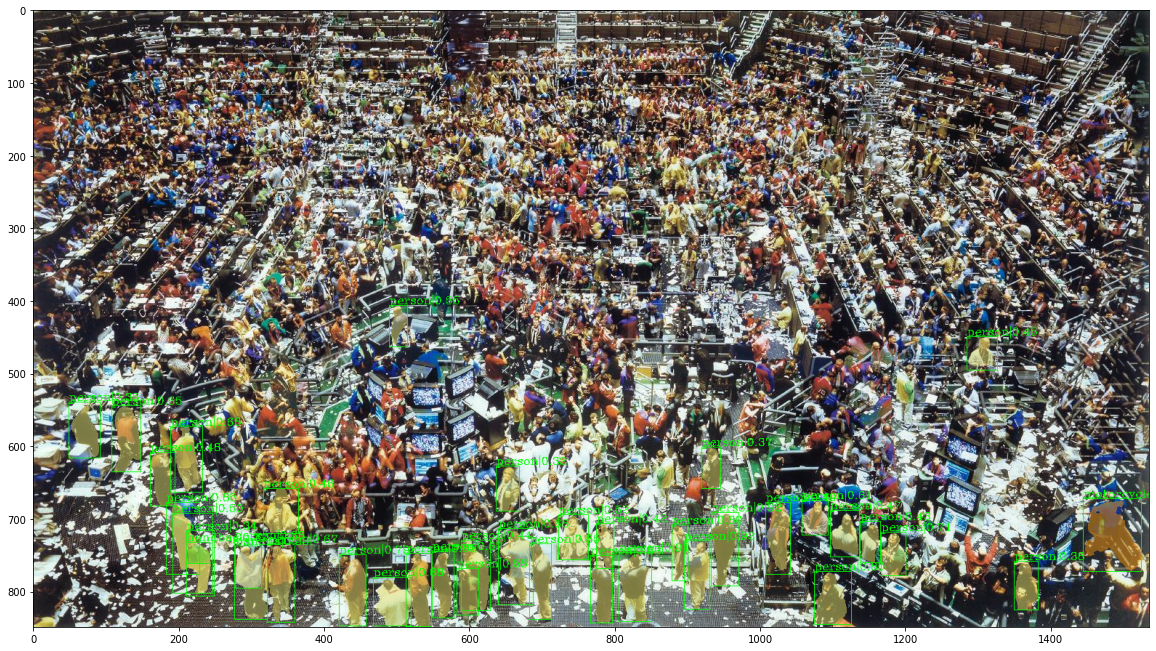
\includegraphics[width=\textwidth]
	{img/gursky-result.png}}
	\caption{\label{fig:fpn} Pretrained model applied on an image from Andreas Gursky}
\end{figure}
	
In sum the performance of the pretrained on COCO-dataset Mask R-CNN model depends on the following criteria: The class of objects depicted in the image (included in COCO-dataset or not), the size of objects in the image and the degree to which an object is visible and is shown in a natural style.

\subsection{Retrained on "Kunst aufräumen" data}

\begin{figure}[H]
\begin{tabular}{cc}
 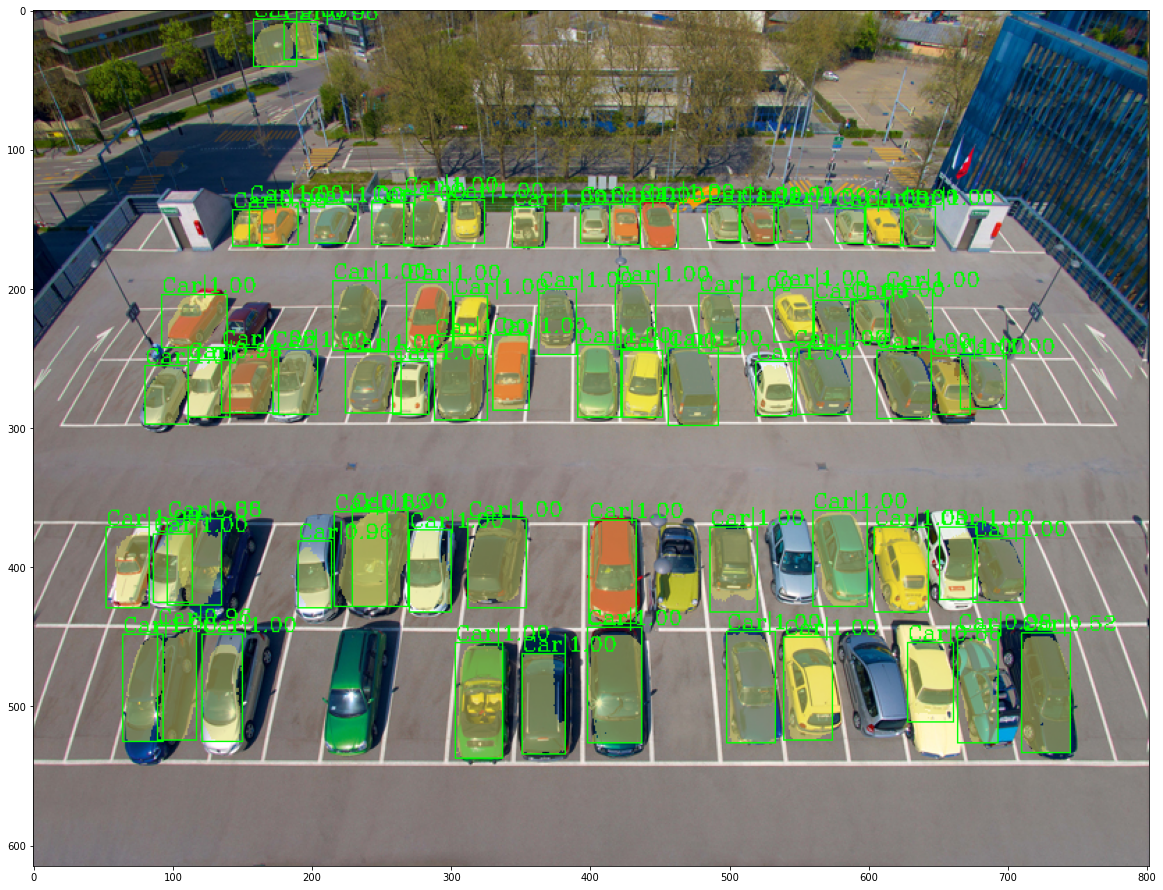
\includegraphics[width=0.5\textwidth]{retrained-only-cars-4500e.png} &   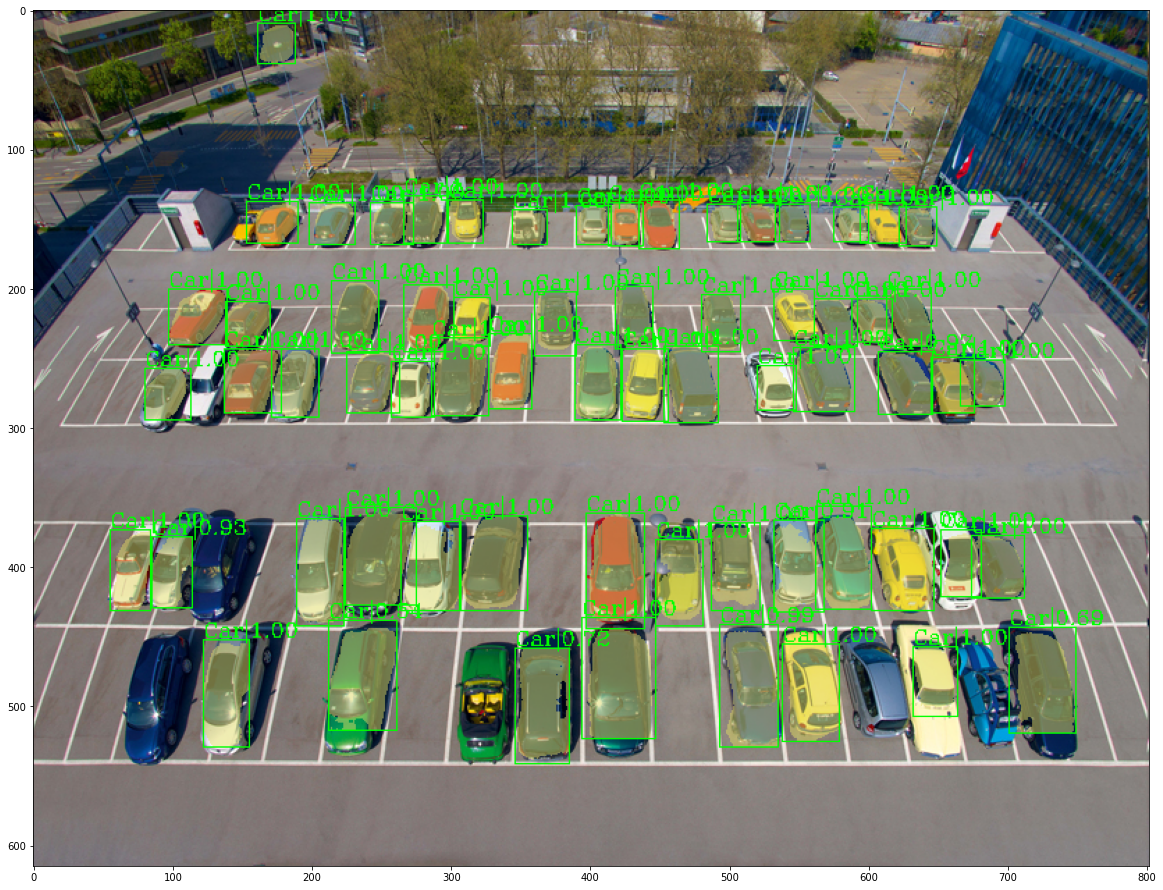
\includegraphics[width=0.5\textwidth]{retrained-only-cars-6000e.png} \\
(a) first & (b) second \\[6pt]
 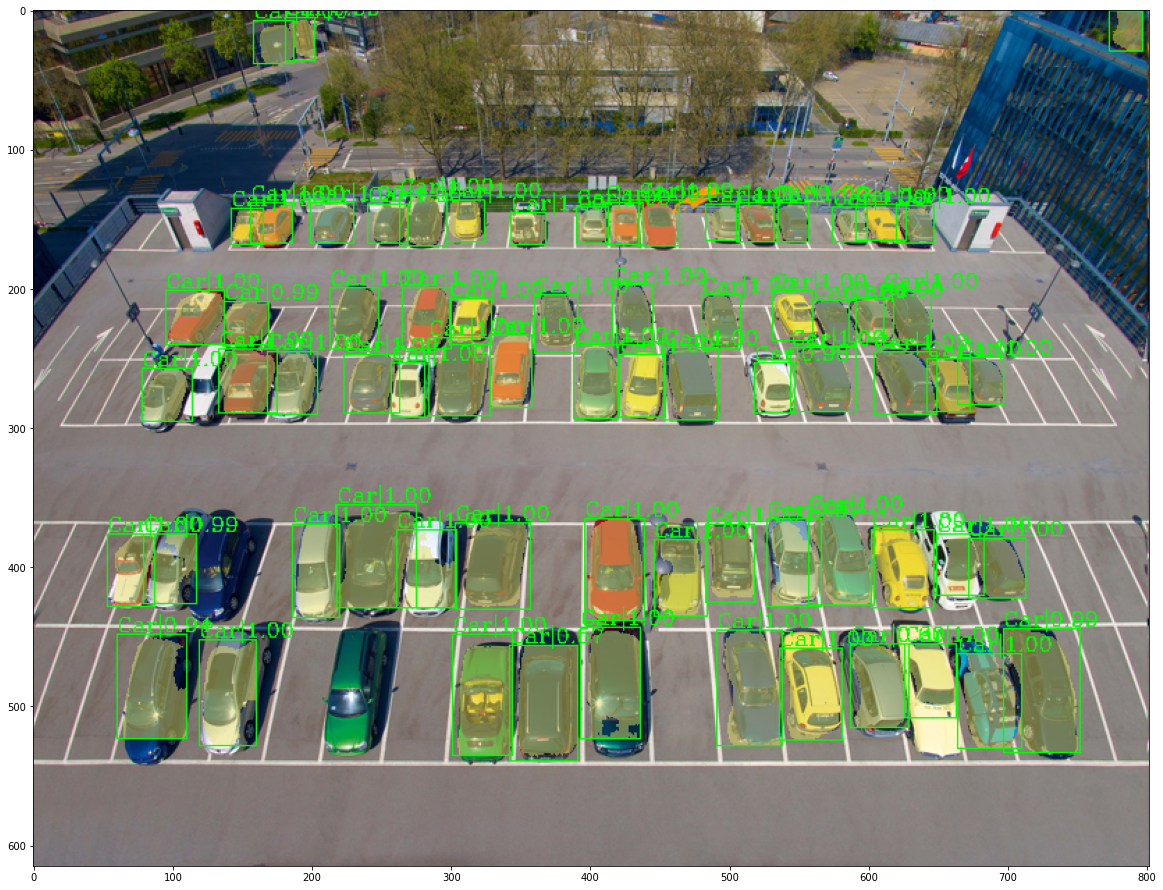
\includegraphics[width=0.5\textwidth]{retrained-only-cars-7500e.png} &   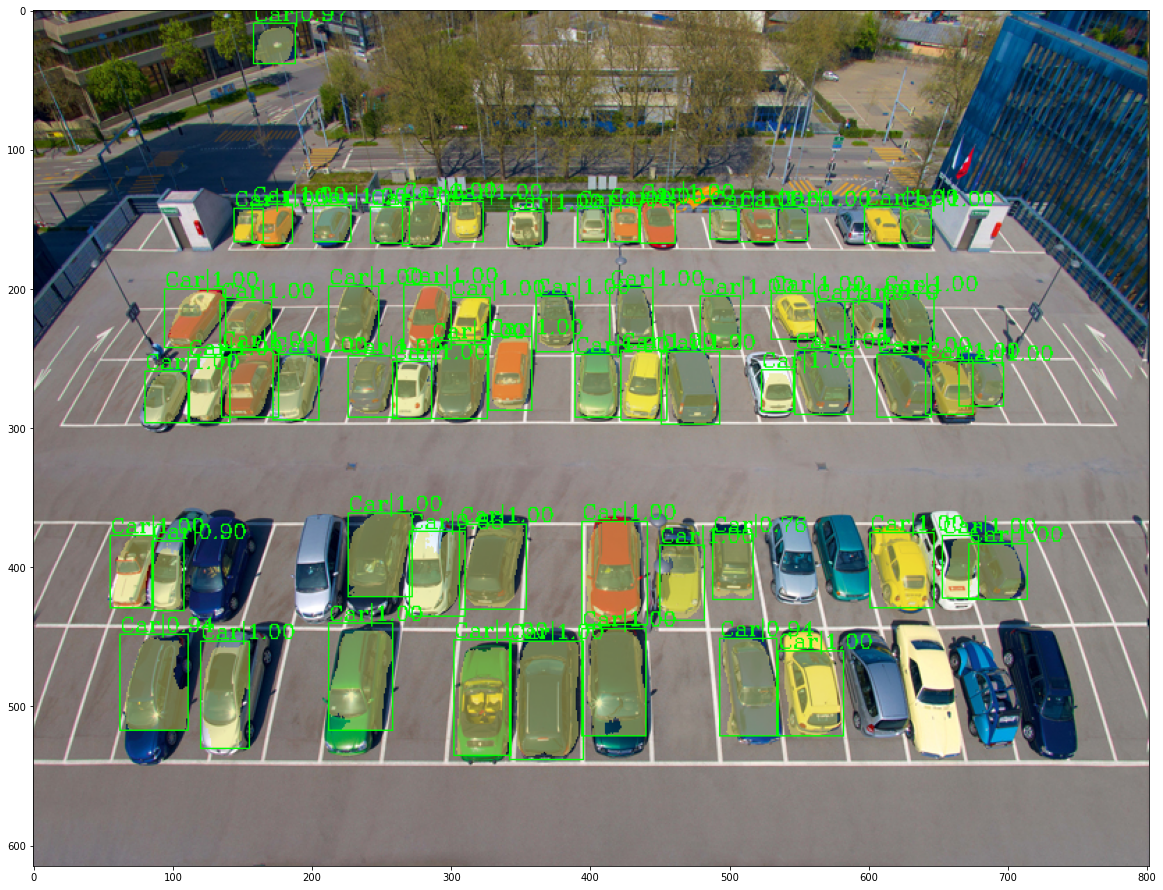
\includegraphics[width=0.5\textwidth]{retrained-only-cars-9000e.png} \\
(c) third & (d) fourth \\[6pt]
\end{tabular}
\caption{Output of the retrained on "Kunst aufräumen" car photo with 4500, 6000, 7500 and 9000 epochs each.}
\end{figure}

\subsection{Web application}

Hello

\section{Comparison with given requirements}

The following tasks could be solved successfully: A dataset, containing of 42 images from four different artist, has been gathered. Different object detection models and frameworks have been tested out on this dataset on Google Colab. The most promising model has been chosen to implement in a web application. The web application has been developed and deployed on the EnterpriseLab successfully. An own model has been created by refining the pretrained on COCO-dataset model on new data from "Kunst aufräumen".

Unfortunately there was no time left to develop an own metric to examine and compare different models when applied to pictures of artistic photography.

\section{Evaluation of technical tools}

Retrospectively, the used tool chain appeared to be very effective. Google Colab is a very powerful infrastracture, especially when one does not possess an own Nvidia GPU. 

MMDetection turned out to be a fast, modular and powerful framework for computer vision projects. Very helpful was the ability to save checkpoints and to resume training in a later point of time. MMDetection got a lot of traction in the last years and is in a steady change, version 2.0.0 just got released in April 2020.

Plotly Dash was a joy to work with, as it lets the developer turn a program into a full-fledged web application very quickly with minimal overhead. As it is built upon JavaScript technologies (React), it is highly customizable too.

Unluckily, to this day, most frameworks do not support operating on CPU in inference mode (however this was fixed in MMDetection 2.0.0). To accomplish this, an indirection via SMD, as explained in \ref{inference-cpu} on page \pageref{inference-cpu} had to be taken. Running the inference on CPU has a major drawback: It slows down computation time badly. To serve a better performance and user experience, a GPU-powered server infrastructure should be considered.

\section{Evaluation of used method}

Hello
